\section{Метод сопряженных градиентов}

\textbf{Алгоритм метода}:
$$ x^{k+1} = x^{k} + t_{k}d^{k}$$
$$ d^{0} = - \nabla f(x^{0})$$
$$ d^{k} = - \nabla f(x^{k}) + \beta_{k - 1}d^{k - 1}$$
$t_{k}$ --- шаг вычисляется из условия наибольшего убывания функции в точках последовательности: $t_{k} = argmin|f(x^{k+1})|$

Основной критерий окончания метода:$|| \nabla f(x^{k})|| < \varepsilon$.

Начальные параметры метода: $x^{0}, \varepsilon$.

Изменяемые параметры метода: отрезок для уточнения шага $[a, b]$.

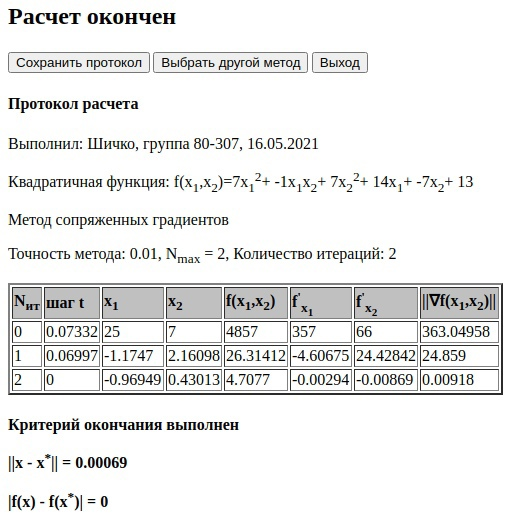
\includegraphics[width=0.8\linewidth]{images/1_prot}\\
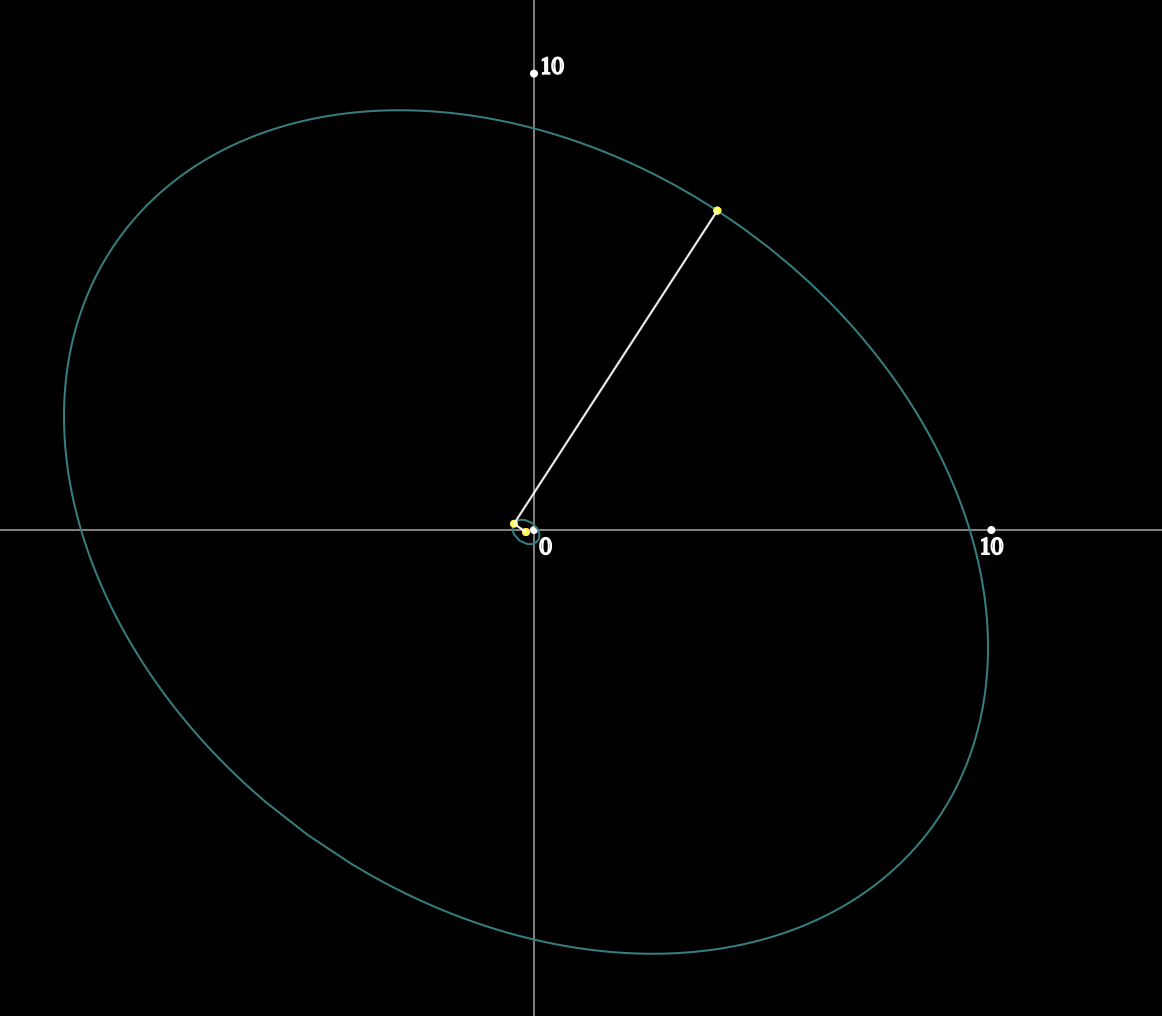
\includegraphics[width=0.6\linewidth]{images/1_graf}\\

\textbf{Последняя итерация}:

$x^{0}_{1} = N^{0} = 4$\\
$x^{0}_{2} = 7$\\
$x^{2} = x^{1} + t_{1} +d^{1}$\\
$
x^{1} = 
\begin{pmatrix}
  -0.4529\\
  0.1438
\end{pmatrix}
$\\
$t_{1} = 0.1274$\\
$d^{1} = -\nabla f(x^{1}) + B_{0}d^{0}$\\
$d^{0} = -\nabla f(x^{0})$\\
$B_{0} = \dfrac{||\nabla f(x^{1})||^{2}}{||\nabla f(x^{0})||^{2}} = \dfrac{(2.5024)^{2}}{(115.663)^{2}} = 0.0046$\\
$
\nabla f = 
\begin{pmatrix}
  10x_{1} - 3x_{2} + 2\\
  12x_{2} - 3x_{1} + 1
\end{pmatrix}
$\\
$
\nabla f(x^{0}) = 
\begin{pmatrix}
  63\\
  97
\end{pmatrix}
$\\
$
\nabla f(x^{1}) = 
\begin{pmatrix}
  -2.097\\
  1.3675
\end{pmatrix}
$\\
Тогда\\
$
d^{1} = 
\begin{pmatrix}
  2.097\\
  -1.3675
\end{pmatrix}
+
\begin{pmatrix}
  -0.2898\\
  -0.4462
\end{pmatrix}
=
\begin{pmatrix}
  1.8072\\
  -1.8137
\end{pmatrix}
$\\

$
x^{2} = 
\begin{pmatrix}
  -0.4529\\
  0.1438
\end{pmatrix}
+ 0.1274
\begin{pmatrix}
  1.8072\\
  1.8137
\end{pmatrix}
=
\begin{pmatrix}
  -0.1829\\
   0.03627
\end{pmatrix}
$
\pagebreak

